% 中身は slides/ を編集する。保存するとこのファイルがビルドされ、pdf/1-1.pdf が更新される。
\documentclass{beamer}
\usepackage{tikz}

\usepackage{luatexja}
\usepackage{luatexja-fontspec}
\usepackage{graphicx}
% 章フォルダの tex/ からコンパイルすることを想定
\graphicspath{{../images/}{images/}}

% ---- ブロックの設定（block / alertblock / exampleblock）----
\definecolor{main}{RGB}{30,70,140}
\definecolor{alertcol}{RGB}{200,80,40}
\definecolor{examplecol}{RGB}{30,120,60}
\setbeamertemplate{blocks}[rounded][shadow=false]

\setbeamercolor{block title}{fg=white,bg=main}
\setbeamercolor{block body}{fg=black,bg=main!6}
\setbeamercolor{block title alerted}{fg=white,bg=alertcol}
\setbeamercolor{block body alerted}{fg=black,bg=alertcol!6}
\setbeamercolor{block title example}{fg=white,bg=examplecol}
\setbeamercolor{block body example}{fg=black,bg=examplecol!6}

\setbeamerfont{block title}{series=\bfseries}
\setbeamerfont{block title alerted}{series=\bfseries}
\setbeamerfont{block title example}{series=\bfseries}

\setbeamertemplate{itemize items}[circle]

\DeclareMathOperator*{\argmax}{arg\,max}
\DeclareMathOperator*{\argmin}{arg\,min}

\author{渡邉 有志}
\date{\today}

\title{The Principles of Diffusion Models}
\subtitle{1.1 What is Deep Generative Modeling?}

\begin{document}

\begin{frame}
    \titlepage
\end{frame}

\begin{frame}{1.1 目次}
    \begin{itemize}
        \item DGMの目標
        \item 順方向KLと最尤推定
        \item Lemma 1.1.1 と Mode Covering
        \item Fisher / f-divergence（JS, TV）
        \item Challenges of Modeling
        \item 補足
    \end{itemize}
\end{frame}

% !TEX root = ../tex/1-1.tex
% DGMとは何か、学習の目標
\begin{frame}{DGM(深層生成モデル)}
\begin{block}{DGM(Deep Generative Models)}
高次元データに対する確率分布を学習し、データセットに類似したサンプルの生成が可能なモデル\\
\end{block}

\vspace{-1em}

\begin{columns}[T]
\begin{column}{0.48\textwidth}
\begin{exampleblock}{\small 目標1 Realistic Generation}
\small 実際のデータと区別できないような\textbf{新しいサンプルを生成}
\end{exampleblock}
\end{column}

\begin{column}{0.48\textwidth}
\begin{exampleblock}{\small 目標2 Controllable Generation}
\small 生成過程を解釈可能な形での制御を可能に
\end{exampleblock}
\end{column}
\end{columns}

\vspace{1em}

\small モデルが表す確率分布:\boldmath{$p_{\phi}$}  実際のデータが従う確率分布\footnote{data distribution, true distributionとも呼び、一般に$p_{data}$自体は未知である}:$p_{data}$\unboldmath\\

\begin{itemize}
\item 有限個のデータセットに対し\\
$p_{\phi}$と$p_{data}$間の損失関数を最小化→${\phi}$を最適化
\end{itemize}

\begin{exampleblock}{}
⇒つまり$p_{\phi}(x)\approx p_{data}(x)$が理想的\\
しかし$p_{data}(x)$が不明なので手元にある$p_{data}$から得られた\\サンプル$x^{(1)},x^{(2)},...x^{(N)}$から$\phi$を学習 ⇒ 分布を推定
\end{exampleblock}
\end{frame}
%=======================================================
\begin{frame}{1.1.1 Mathematical Setup -Goal of DGM}
\begin{exampleblock}{}
    前提：未知の分布$p_{data}$からサンプリングした有限個のサンプル\[
\left\{\mathbf{x}^{(i)}\right\}_{i=1}^{N}が手元にある
\]
\end{exampleblock}
\small $p_{data}$を表す式、新しいサンプルを生成する方法もわからない\\
⇒そこでパラメータ$\phi$を持つ深層ネットで\textbf{モデル分布}$p_{\phi}(x)$を構成\footnote{pは文脈により($p_{data}$)確率分布または($p_{data}(x)$)確率密度関数}
\begin{block}{DGMの目標}
    \centering$\phi^{*}$を学習して$p_{\phi^{*}}(\boldsymbol{x})\approx p_{data}(\boldsymbol{x})$\\
    $p_{\phi}$をGenerative model（生成モデル）という
\end{block}
⇒未知の$p_{data}$から得られた有限データを使って$p_{\phi^{*}}\approx p_{data}$となる\\
モデルを学習し、そこから新しいデータを生成する\\
\vspace{1em}
\textbf{生成}：学習済みの分布から新しいサンプルをサンプリングすること\\
\centering $\boldsymbol{x}\sim p_{\phi}$とすると$\boldsymbol{x}$は新しいサンプル

\end{frame}
%=======================================================
\begin{frame}{Figure 1.1：DGMの目標}
    \centering
    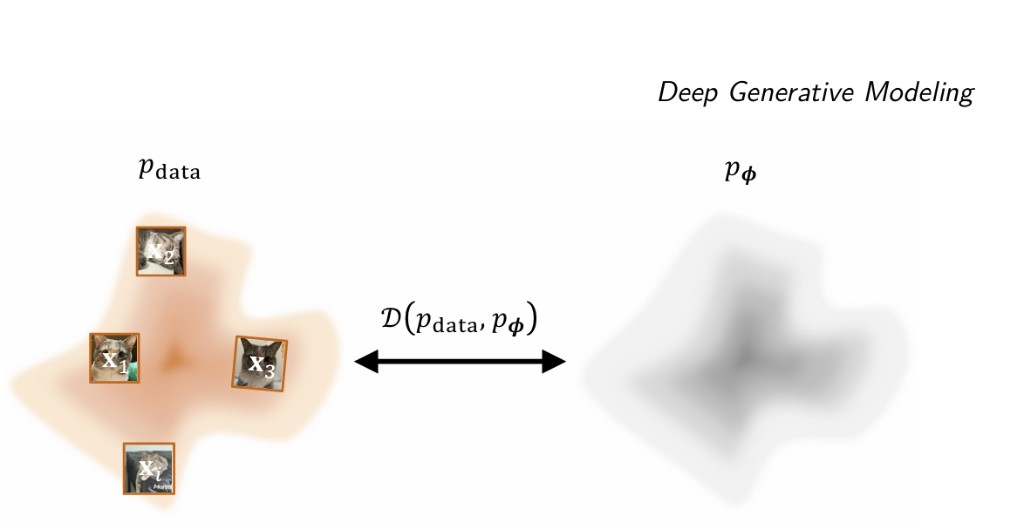
\includegraphics[
        width=\textwidth,
        height=0.55\textheight,
        keepaspectratio
    ]{figure1-1.png}
    \begin{exampleblock}{目的}
    モデル分布$p_{\phi}(x)$とデータ分布$p_{data}(x)$の隔たりを最小化\\
    \end{exampleblock}
    \small 未知の分布$p_{\mathrm{data}}(x)$から得た有限個の独立同分布（i.i.d.）サンプル$\{\boldsymbol{x}^{(i)}\}_{i=1}^{N}$を用いて$\phi$を学習し、新たなサンプルを生成する。

\end{frame}

% !TEX root = ../tex/1-1.tex
% 学習の定式化と順方向KL
\begin{frame}{1-1-1 Training of DGM}
\begin{block}{学習}
モデル族$\{p_{\phi}\}$の中で不一致$\mathcal{D}$を最小化するパラメータを求める\\
\centering $\phi^{*}\in \argmin_{\phi}\mathcal{D}(p_{data},p_{\phi})$
\end{block}
\begin{itemize}
\item $\boldsymbol{p}_{data}$は、未知であるためi.i.d.サンプルから値を効率的に\\
推定することによって実用的なDを選ぶ\\
\item モデルに十分な表現力があれば$\boldsymbol{p}_{data}$と$\boldsymbol{p}_{\phi}$の近似ができる\\
\end{itemize}

\begin{block}{順方向KL divergenceと最尤推定}
    MLE(Maximum Likelihood Estimation): 最尤推定\\
    ⇒訓練データから最も尤もらしいパラメータ$\phi^{*}$を推定する方法\\
    \small ※モチベーション：モデルの確率密度$p_{\phi}(x)$を評価できる場合、観測されたデータに対してモデルが高い確率密度を与えるパラメータを選ぶ\\
\end{block}

\end{frame}
%=======================================================
\begin{frame}{Forward KL divergence}
\begin{block}{定義:KL divergence}
    \begin{align*}
        D_{KL}(p_{data}\mid\mid p_{\phi})
        &:= \int p_{data}(\boldsymbol{x})\log\frac{p_{data}(\boldsymbol{x})}{p_{\phi}(\boldsymbol{x})}\,dx \\
        &= \mathbb{E}_{\boldsymbol{x}\sim p_{data}}
            [\log p_{data}(\boldsymbol{x})-\log p_{\phi}(\boldsymbol{x})]
        \end{align*}
        二つの確率分布の隔たりを測る指標
\end{block}

\begin{itemize}
    \item 非対称\footnote{||は二つの確率分布を区別し、慣用的に非対称を表すこともある}:$D_{KL}(p_{data}\mid p_{\phi} )\neq D_{KL}(p_{\phi}\mid\mid p_{data})$
    \item 非負性:$D_{KL}(p_{data}\mid\mid p_{\phi})\geq 0$
    \item 一致時に0:$D_{KL}(p_{data}\mid\mid p_{\phi})=0$⇔$p_{data}=p_{\phi}$
\end{itemize}

\end{frame}
%=====================================================
\begin{frame}{さらに分解すると}
    \begin{block}{}
        一見すると、データの確率密度 \(p_{\mathrm{data}}(x)\) が未知であるため、\\
        順方向のKLダイバージェンスは利用できなそうだが
        \begin{align*}
            D_{\mathrm{KL}}(p_{\mathrm{data}}\mid\mid p_{\phi})
            &= \mathbb{E}_{x\sim p_{\mathrm{data}}}
                \left[
                    \log\frac{p_{\mathrm{data}}(x)}{p_{\phi}(x)}
                \right] \\
            &= -\mathbb{E}_{x\sim p_{\mathrm{data}}}
                \bigl[\log p_{\phi}(x)\bigr]
                - H(p_{\mathrm{data}}).
        \end{align*}
        ここで
        \[
            H(p_{\mathrm{data}})
            :=
            -\mathbb{E}_{x\sim p_{\mathrm{data}}}
            \bigl[\log p_{\mathrm{data}}(x)\bigr].
        \]
        \small はデータ分布のエントロピーと呼ばれ、パラメーター$\phi$に依存しない定数
    \end{block}
\end{frame}

% !TEX root = ../tex/1-1.tex
% KLの意味、最尤推定との同値、Mode Covering
\begin{frame}{KLダイバージェンスのモチベーション(1)}
    \small モデルの分布が真の分布をどれだけ適切に表現できているかを測る指標
    \begin{block}{なぜ確率の比を考えるか}
    あるデータxについて$\log \frac{p_{data}(x)}{p_{\phi}(x)}$を考える\\
    ⇒同じｘに対してどの程度の確率（確率密度）を割り当てているか\\
    \end{block}
    \begin{block}{対数を使う理由}
        離散データでは確率$p(x)$に対して$-\log p(x)$は情報量を表す\\
    \[
\log\frac{p_{\mathrm{data}}(x)}{p_{\phi}(x)}
=
\underbrace{-\log p_{\phi}(x)}_{\text{モデルに基づく情報量}}
-
\underbrace{\bigl(-\log p_{\mathrm{data}}(x)\bigr)}_{\text{本当の分布に基づく情報量}}
\]
    \end{block}

    \begin{block}{なぜデータ分布で平均するのか}
        1つのxだけでは分布が適切かどうか判断できない\\
        ⇒データ分布で平均することで分布が適切かどうか判断できる\\
        \centering$D_{KL}(p_{data}\mid\mid p_{\phi})=\mathbb{E}_{\boldsymbol{x}\sim p_{data}}[\log \frac{p_{data}(\boldsymbol{x})}{p_{\phi}(\boldsymbol{x})}]$\\
        連続値の場合は期待値を積分で書く\\
        ここで、重み$p_{data}$は実データで現れる領域での評価を平均に強く反映
    \end{block}

\end{frame}
%=======================================================
\begin{frame}{KLダイバージェンスのモチベーション(2)}
    なぜ数学的な距離\footnote{数学的な距離は正値性、対称性、三角不等式を満たす性質を持つ}を使わないのか
    \begin{itemize}
    \item 分布の違いの評価が可能\\
    ⇒数学的な距離は満たさないが、非負で0になるのは両分布が一致するときであり目的関数として利用できる\\
    \item 実データを基準にして評価できる\\
    ⇒比較に方向があり、実データで起こりやすいものにモデルが低い確率を割り当てると、大きなペナルティ
    \item 最尤推定につなげやすい\\
    ⇒順方向KLの最小化は、対数尤度の期待値の最大化と同じ
    \item 未知のデータ分布でも学習可能\\
    ⇒期待値をサンプル平均で近似すれば、手元の訓練データとモデルの確率密度を使って学習可能

    \end{itemize}

\end{frame}
%=======================================================
\begin{frame}{Lemma. 1.1.1}
\begin{exampleblock}{Lemma 1.1.1 (Minimizing KL $\leftrightarrow$ MLE)}
    \centering$\min\limits_{\phi}\mathcal{D}(p_{data}\mid\mid p_{\phi})\iff \max\limits_{\phi}\mathbb{E}_{x\sim p_{data}}[\log p_{\phi}(x)]$
\end{exampleblock}
\vspace{1em}
$p_{data}$の期待値をサンプル${\boldsymbol{x}^{(i)}}_{i=1}^{N}$を用いた平均に置き換え\\
ただし、$p_{data}$からi.i.d.で抽出したと仮定する。\\
これにより経験的な負の対数尤度を目的関数として得る
\vspace{1em}
\centering$\hat{\mathcal{L}}_{MLE}(\phi) := -\frac{1}{N}\sum_{i=1}^{N}\log p_{\phi}(x^{(i)})$\\
\vspace{1em}
ミニバッチから計算した確率的勾配法を用いて最適化が可能\\
⇒最尤推定に必要なのは$p_{data}$から得られたサンプルのみであり、\\未知のデータ分布の確率密度そのものを評価しなくてよい

\end{frame}
%=======================================================
\begin{frame}{証明}
    \begin{exampleblock}{証明(lemma1.1.1)}
エントロピー等の各項が有限で最適解が存在すると仮定する

\centering$\mathcal{J}(\phi) := \mathbb{E}_{x\sim p_{data}}[\log p_{\phi}{x}]$と置くと
\centering$\mathcal{D}_{KL}(p_{data}\mid\mid p_{\phi}) = \mathcal{J}(\phi) + H(p_{data})$\\
\small ※ここで、$\mathcal{H}は\phi$に依存しない定数である\\
\end{exampleblock}

\begin{exampleblock}{}
    ($\implies$)
$\phi^{*}$がKLを最小にすると仮定すると
\centering$\forall \phi,\mathcal{D}_{KL}(p_{data}\mid\mid p^{\phi^{*}}) \leq \mathcal{D}_{KL}(p_{data}\mid\mid p^{\phi})$
\centering$-\mathcal{J}(\phi^{*})-\mathcal{H}(p_{data}) \leq -\mathcal{J}(\phi)-\mathcal{H}(p_{data})$\\
\centering$-\mathcal{J}(\phi^{*}) \leq -\mathcal{J}(\phi)$\\
\centering$\mathcal{J}(\phi^{*}) \geq \mathcal{J}(\phi)$\\
任意の$\phi$に対して成り立つため、$\phi^{*}$は期待対数尤度を最大にする
\end{exampleblock}

\begin{exampleblock}{}
($\impliedby$)
$\phi^{*}$が期待対数尤度を最大にすると仮定すると
\centering$\forall \phi,\mathcal{J}(\phi^{*}) \geq \mathcal{J}(\phi)$\\
さっきの逆の手順によって証明可能\\
任意の$\phi$に対して成り立つため、$\phi^{*}$はKLを最小にする
\end{exampleblock}
\end{frame}
%=======================================================
\begin{frame}{順方向のKLダイバージェンス}
    \begin{block}{}
    \centering$\mathcal{D}_{KL}(p_{data}\mid\mid p_{\phi})=\mathbb{E}_{x\sim p_{data}}[\log \frac{p_{data}(x)}{p_{\phi}(x)}]$

        \begin{itemize}
            \item 順方向\\
            データ分布に関して期待値を取る\\
            ⇒$p_{data}$の下でデータが現れる領域をモデルも捉える必要
            \item 逆方向\\
            モデル分布から得られるサンプルに関して期待値を取る
        \end{itemize}

        \begin{alertblock}{Mode Covering}
            データ分布が正の確率を割り当てる領域をAとする\\
            すなわち$p_{data}(A)>0$が存在するがモデルが密度を割り当てずに$x\in A$に対して($p_{\phi}(x)=0$)であるとする\\
            このとき$p_{data}(x)>0$ である場所では\\
            \centering$\log \frac{p_{data}(x)}{p_{\phi}(x)}=+\infty$\\

            データ分布が確率密度を割り当てた領域を見落とす場合に\\強いペナルティを与える
            ⇒Mode Covering(モード被覆)
        \end{alertblock}
    \end{block}
\end{frame}

% !TEX root = ../tex/1-1.tex
% Fisher、f-divergence、JS、TV
\begin{frame}{Fisher Divergence}
    \begin{block}{定義:Fisher Divergence}
    \centering$\mathcal{D}_{F}(p\mid\mid q):=\mathbb{E}_{x\sim p}[||\nabla_x \log p(x)-\nabla_x \log q(x)||_{2}^{2}]$  \\
    スコア関数$\nabla_x \log p(x)$の隔たりを測る\\
    スコア関数は確率密度がより高い領域に向かうベクトル場である

\end{block}

    \begin{itemize}
        \item $\mathcal{D}_{F}(p\mid\mid q) \geq0$\\
        ⇒等号成立は$p=q$のとき\footnote{密度の滑らかさ、共通の台の連結性が必要}、対数密度の一致を意味する勾配にのみ依存し、正規か定数に依存しない\footnote{密度に掛かる定数が対数の勾配を取ると消える} \\
        \item スコアマッチングの基礎となる\\
        ⇒生成のために対数尤度の勾配を学習する方法\\
        \item データ分布$p=p_{data}$が目標になり、モデル$q=p_{\phi}$はデータ分布のスコア場に一致させるように学習\\
    \end{itemize}


\end{frame}
%=======================================================
\begin{frame}{KL以外の尺度}
    \begin{block}{f-divergence}
        \centering$\mathcal{D}_{f}(p\mid\mid q):=\int q(x)\mathit{f}\left(\frac{p(x)}{q(x)}\right)dx$\\
        ここで、$\mathit{f}: \mathbb{R}_{+} \to \mathbb{R}$は凸関数で、$\mathit{f}(1)=0$を満たす。\\
        $\mathit{f}$を変えることで様々なダイバージェンスを定義できる。
    \end{block}
    \centering
\begin{tikzpicture}
  \draw[thick, fill=blue!5] (0,0) ellipse (4cm and 2cm);
  \node at (0,1.35) {$f$-divergence};
  \node[draw, thick, circle, fill=white, minimum size=1.2cm] at (-2,-0.2) {KL};
  \node[draw, thick, circle, fill=white, minimum size=1.2cm] at (0,-0.2) {JS};
  \node[draw, thick, circle, fill=white, minimum size=1.2cm] at (2,-0.2) {TV};
\end{tikzpicture}


\end{frame}
%=======================================================
\begin{frame}{f-divergenceとKL-divergenceの関係}
    \begin{exampleblock}{forward KL}
        \centering$\mathit{f}(u)=u\log u \implies \mathcal{D}_{f}=\mathcal{D}_{KL}(p\mid\mid q)$\\
    \end{exampleblock}
    \begin{exampleblock}{}
    \centering$ \mathcal{D}_{f}(p\mid\mid q)=\int q(x)\mathit{f}\left(\frac{p(x)}{q(x)}\right)dx$\\
    \centering ここで$\mathit{f}(u)=u\log u$とすると、\\
    \begin{align*}
        \mathcal{D}_{f}(p\mid\mid q)
        &= \int q(x)\,f\Bigl(\frac{p(x)}{q(x)}\Bigr)\,dx \\
        &= \int q(x)\frac{p(x)}{q(x)}\log\frac{p(x)}{q(x)}\,dx \\
        &= \int p(x)\log\frac{p(x)}{q(x)}\,dx \\
        &= \mathcal{D}_{\mathrm{KL}}(p\mid\mid q)
    \end{align*}
    \end{exampleblock}
\end{frame}

%=======================================================
\begin{frame}{Jensen-Shannon divergence}
    \begin{exampleblock}{Jensen-Shannon}
        \centering$\mathit{f}(u)=\frac{1}{2}[u\log u-(1+u)\log\frac{(1+u)}{2}] \implies \mathcal{D}_{f}=\mathcal{D}_{JS}(p\mid\mid q)$\\
    \end{exampleblock}
        \begin{itemize}
        \item 対称性を持つ
        \item 非負性を持つ
        \item 一致時に0になる
    \end{itemize}
    $f(1)=0$は両分布が一致したときに評価値を0にするための条件\\
    凸関数であることは非負性を保証する\\
    $P(x)>0$ならば$m(x)>0$なのでKLのように比較先の密度が\\ゼロだから無限大になることはない


    \end{frame}
%=======================================================
\begin{frame}{f-divergenceとJensen-Shannon divergenceの関係}
    \begin{exampleblock}{}
    \small
    $\mathit{f}(u)=\dfrac{1}{2}\bigl[u\log u-(1+u)\log\dfrac{1+u}{2}\bigr]$
    とすると、
    \begin{align*}
    \mathcal{D}_{f}(p\mid\mid q)
    &= \int q(x)\,
       f\Bigl(\frac{p(x)}{q(x)}\Bigr)\,dx \\
    &= \frac{1}{2}\int
       \Bigl[
         p(x)\log\frac{p(x)}{q(x)}
         -(p(x)+q(x))\log\frac{p(x)+q(x)}{2q(x)}
       \Bigr]dx
    \end{align*}
    二つの分布の平均を
    $m(x)=\dfrac{p(x)+q(x)}{2}$
    とすると、
    \begin{align*}
        & p(x)\log\frac{p(x)}{q(x)}
          -(p(x)+q(x))\log\frac{m(x)}{q(x)} \\
        &= p(x)\Bigl[
             \log\frac{p(x)}{q(x)}
             -\log\frac{m(x)}{q(x)}
           \Bigr]
           -q(x)\log\frac{m(x)}{q(x)} \\
        &= p(x)\log\frac{p(x)}{m(x)}
           -q(x)\log\frac{m(x)}{q(x)}
        \end{align*}
        \centering$\therefore \mathcal{D}_{JS}(p\mid\mid q)=\frac{1}{2}\mathcal{D}_{KL}(p\mid\mid m)+\frac{1}{2}\mathcal{D}_{KL}(q\mid\mid m)$
    \end{exampleblock}
    \end{frame}
%=======================================================
\begin{frame}{total variation}
    \begin{exampleblock}{total variation}
        \centering$\mathit{f}(u)=\frac{1}{2}|u-1| \implies \mathcal{D}_{f}=\mathcal{D}_{TV}(p\mid\mid q)$\\
    \end{exampleblock}
    二つの分布の間で生じうる最大の確率の差を捉える尺度\footnote{別の見方として代表的な尺度ワッサーシュタイン距離(7章で扱う)}
    \begin{columns}[T]
        \begin{column}{0.48\textwidth}
            \begin{itemize}
                \item 対称性を持つ
                \item 非負性をもつ
            \end{itemize}
        \end{column}
        \begin{column}{0.48\textwidth}
            \begin{itemize}
                \item 一致時に0になる
                \item 三角不等式を満たす
            \end{itemize}
        \end{column}
    \end{columns}

    \begin{exampleblock}{}
    $\mathit{f}(u)=\frac{1}{2}|u-1|$とすると、
    \begin{align*}
        \mathcal{D}_{f}(p\mid\mid q)
        &=\frac{1}{2}\int q(x)|\frac{p(x)}{q(x)}-1|dx\\
        &=\frac{1}{2}\int q(x)|\frac{p(x)-q(x)}{q(x)}|dx\\
        &=\frac{1}{2}\int |p(x)-q(x)|dx\\
    \end{align*}
    \end{exampleblock}
\end{frame}

% !TEX root = ../tex/1-1.tex
% Challenges of Modeling
\begin{frame}{分布のモデリングにおける課題}
    ★複雑なデータ分布をモデル化するためにNNを用いて$p_{data}$を近似するためのモデル分布$p_{\phi}$をパラメータ化したい\\
    \begin{block}{$p_{\phi}$が有効な確率密度になるための条件}
        \begin{itemize}
            \item[(i)] 非負性：$\forall x, p_{\phi}(x)\geq 0$
            \item[(ii)] 正規化：$\int p_{\phi}(x)dx=1$
        \end{itemize}
    \end{block}
    NNは入力xに対して実数のスカラー$\mathit{E}_{\phi}(x)\in \mathbb{R}$を出力する\\
    この出力を有効な確率密度として以下の方法で解釈したい\\
    \begin{itemize}
        \item[①] 条件(i)(ii)を満たす
        \item[②] $\mathit{E}_{\phi}:\mathbb{R}^D\to \mathbb{R}$を未正規化密度を定める関数として捉える
    \end{itemize}
\end{frame}
%=======================================================
\begin{frame}{ステップ1:非負性の保証}
    NNの未加工の出力$\mathit{E}_{\phi}(x)$に、非負の関数を適用する\\
    例：$|\mathit{E}_{\phi}(x)|$や$\mathit{E}_{\phi}(x)^{2}$\\
    ⇒モデルの出力が常に非負になる
    \begin{exampleblock}{標準的な選択：指数関数}
        常に正となる未正規化密度$\widetilde{p}_{\phi}(x)$が得られる
        \[
            \widetilde{p}_{\phi}(x)=\exp(\mathit{E}_{\phi}(x))
        \]
    \end{exampleblock}
    \small ※指数関数だけでは、積分が有限になることまでは保証されない
\end{frame}
%=======================================================
\begin{frame}{ステップ2:正規化}
    $\widetilde{p}_{\phi}(x)$は正だが、積分が$1$になるとは限らない\\
    ⇒空間全体の積分で割って、有効な確率密度にする
    \[
        p_{\phi}(x)
        =\frac{\widetilde{p}_{\phi}(x)}{\int\widetilde{p}_{\phi}(x')\,dx'}
        =\frac{\exp(\mathit{E}_{\phi}(x))}{\int\exp(\mathit{E}_{\phi}(x'))\,dx'}
    \]
    \begin{block}{正規化定数（分配関数）}
        \[
            Z(\phi):=\int\exp(\mathit{E}_{\phi}(x'))\,dx'
        \]
        有効な確率密度になるのは$0<Z(\phi)<\infty$のとき
    \end{block}
\end{frame}
%=======================================================
\begin{frame}{正規化定数の計算困難}
    \begin{alertblock}{計算上の課題}
        高次元では$Z(\phi)$の積分を現実的な計算量で求められない\\
        ⇒この困難さが、様々な深層生成モデルのモデル族を生む中心的な問題
    \end{alertblock}
    以降の節では、正規化定数の評価を回避するか、\\
    計算費用を減らすように設計された主要なアプローチを紹介する
\end{frame}
%=======================================================


% !TEX root = ../tex/1-1.tex
% 補足：i.i.d. と大数の法則
\begin{frame}{補足i.i.d(independent and identically distributed)}
    \begin{block}{i.i.d(independent and identically distributed)}
        独立同分布(i.i.d.): 各サンプルが互いに独立で、同じ分布から生成される
        \begin{itemize}
            \item 独立とは、あるサンプルの値が他のサンプルの値に影響を与えないこと
            \item 同分布とは、すべてのサンプルが同じ分布から生成されること（同じ分布$\neq$同じ値）
        \end{itemize}
    \end{block}
    \begin{block}{i.i.d.の例}
        \[
            p(x^{(1)},\ldots,x^{(N)})
            =\prod_{i=1}^{N}p_{\mathrm{data}}(x^{(i)})
        \]
    \end{block}
\end{frame}
%=======================================================
\begin{frame}{補足：大数の法則}
    \begin{block}{大数の法則}

        独立同分布に従う確率変数の平均は、サンプル数を増やすと真の平均に近づく\\

        \centering$\lim_{N\to\infty}P(|\frac{X_{1}+X_{2}+...+X_{N}}{N}-\mu|\geq \epsilon)=0$
    \end{block}
\end{frame}


\end{document}
